\chapter{Introduction}
\section{Problem statement}
Due to the damaging environmental effects of using fossil fuels in the transport sector, national and 
international targets have been set in order to reduce global CO\textsubscript{2} emissions.
In the UK for example, there is a plan to completely ban the sale of new conventional petroleum vehicles 
by as early as 2040. 
\cite{DepartmentforEnvironment2017} 
One proposed solution is further adoption of fuel cells and other energy generation methods which utilize
hydrogen as a carbon free energy source. 

Despite the fact that the technology for hydrogen powered fuel vehicles has existed since the early 1960’s, their application has been limited to providing power for space missions and other niche applications. In the late 90’s developments in lowering the platinum catalyst loading and breakthroughs in the production of thin film electrodes drove the cost of fuel cells down to a level where they were commercially viable for other applications. As of 2017, a number of auto mobile manufacturers including Toyota,\cite{Toyota2015} Hyundai, \cite{Hyundai2015} Honda \cite{Honda} and Daimler \cite{Mohrdieck2014} now offer hydrogen vehicles commercially. It is also possible to retrofit a petroleum vehicle to run off hydrogen.\cite{FCell2016} Many countries both in the EU, and globally have ambitious hydrogen infrastructure plans over the next 10 years. This is in an effort to become less reliant on importing fossil fuels, increase their energy security, and transition to a carbon free energy system.

The development of the hydrogen economy is still in its infancy,  however several countries are aiming to deploy sizable hydrogen fuelling infrastructures over the next few decades. National reports state that Europe’s position in 2030 will be: UK - 1,100 hydrogen refuelling stations and 1.6 million fuel cell vehicles \cite{UKH2Mobility2013} France – 600 hydrogen refuelling stations and 0.8 million fuel cell vehicles \cite{Summerton2015}, Germany – 1,180 hydrogen refuelling stations \cite{Hayter2014} and 1.8 million fuel cell vehicles  and the Netherlands – 200 hydrogen refuelling stations and 0.2 million fuel cell vehicles. \cite{Hayter2014} Although this report seems to have overestimated the development, for example as of 2020 the UK only has 17 HRS's \cite{stephen_errity_2020}, compared to the 65 estimated by the report.  

The fuel cell system in a hydrogen vehicle can easily degrade if even parts-per-billion to parts-per-million level of some impurities are present in the hydrogen. Therefore, it is imperative that hydrogen purity, and techniques for verifying purity, are adequate to ensure customers vehicles are not inadvertently damaged by fluctuations in hydrogen composition. International standards advise that all hydrogen suppliers should prove that their product is pure enough to prevent degradation of fuel cell components. ISO 14687 \cite{InternationalStandardISO14687-2:20122012}, shown in Table \ref{tab:1} specifies the maximum impurity levels of 13 impurities that are permissible in fuel cell hydrogen. ISO 14687 includes some challenging hydrogen purity specifications mainly due to the impurity limits being below the limits of detection of the standard techniques commonly used to measure the concentration of these compounds. 

\begin{table}[]
    \caption{Concentration limits for ISO-14687 impurities}
    \centering
    \begin{tabular}{@{}cc@{}}
    \toprule
    \textbf{Characteristics}                  & \textbf{Regulation}    \\ \midrule
    Minimum mole fraction of hydrogen         & 99.97\%                \\
    Total non-hydrogen gases                  & 300 µmol mol-1         \\ \midrule
    \multicolumn{2}{c}{\textbf{Maximum concentration of individual components}} \\ \midrule
    Total Hydrocarbons (Methane basis)        & 5 µmol mol-1           \\
    Water                                     & 2 µmol mol-1           \\
    Oxygen                                    & 5 µmol mol-1           \\
    Helium                                    & 300 µmol mol-1         \\
    Carbon dioxide                            & 2 µmol mol-1           \\
    Carbon monoxide                           & 0.2 µmol mol-1         \\
    Total sulphur compounds (H\textsubscript{2}S basis)       & 0.004 µmol mol-1       \\
    Formaldehyde                              & 0.01 µmol mol-1        \\
    Formic acid                               & 0.2 µmol mol-1         \\
    Ammonia                                   & 0.1 µmol mol-1         \\
    Total halogenated compounds               & 0.05 µmol mol-1        \\
    Maximum particulate concentration         & 1 mg/kg                \\ \bottomrule
    \end{tabular}
    \label{tab:1}
\end{table}

Commercial hydrogen purity laboratories are unable to perform traceable analysis to ISO 14687 
specifications because appropriate methods and standards have not been developed. The consequence 
of this is that hydrogen suppliers cannot provide evidence that their fuel meets these specifications and therefore are not permitted to supply hydrogen. Of the 13 gaseous impurities listed in 
ISO 14687  there is no single method for measuring all impurities. Laboratories must therefore use 
several instruments to perform such an analysis.  In 2015 Murugan et al published a review of methods 
for analysing the purity of fuel grade hydrogen \cite{Murugan2015}. They concluded that in order for a single laboratory to provide full hydrogen analysis to ISO 14687 specifications it would require 
a number of instruments including Gas Chromatography (GC), Fourier-transform infrared spectroscopy (FTIR) and Cavity ring-down spectroscopy (CRDS). The capital cost of purchasing the gas 
analysers to perform analysis on the measurable impurities in a hydrogen sample can amount to 
$>$€500,000 \cite{Murugan2015} and hence performing analysis would be out of reach for many 
laboratories. 

While the impurities listed in ISO 14687 are specified at extremely low amount fractions, 
many can be analysed at higher amount fractions through the use of cheap and routine gas 
analysers such as Gas Chromatography - Mass Spectrometry (GC-MS). A potential solution is, instead of measuring the concentration of each impurity directly using costly and specialised pieces of equipment, to increase the concentration of impurities above the limit of detection of a cheaper, more widespread analyser. These techniques are referred 
to as enrichment or pre-concentration. The most commonly used technique for pre-concentration 
of hydrogen fuel samples is referred to as ‘Hydrogen Impurity Enrichment’. This method involves 
passing the sample through a semi permeable membrane material, such as palladium, which only allows the passage of hydrogen.\cite{NathanW.Ockwig2007a} As hydrogen leaves the system, the impurities remain, increasing in concentration with time as more hydrogen permeates through the membrane. This increase in concentration is referred to as the enrichment factor and once the enrichment is complete the sample can then be analysed at these higher concentrations, and using the enrichment factor, the original composition of the sample can be found. 

The accuracy, cost and time taken for a hydrogen enrichment device is highly dependent on the membrane material. Different materials will allow hydrogen to permeate at different rates and will interact differently with impurities that may be present in hydrogen.\cite{NathanW.Ockwig2007a} While hydrogen enrichment is a promising technology for hydrogen impurity measurement, more research must be done to properly understand how different membrane materials interact with common hydrogen impurities, and therefore identify the most appropriate material.

\section{Research Objectives}
The issue with past enrichment studies are mainly due to the membrane used. Current commercial membranes suffer from low flux values, driving up the enrichment time, and are highly reactive with hydrogen impurities which throws off the results. This thesis will focus on developing and improving hydrogen impurity enrichment as a method for measuring the impurities in fuel grade hydrogen to ISO 14687. Studies will revolve around the membrane materials used to concentrate the impurities in hydrogen samples, optimisation of process parameters, and improvements of the enrichment device. The final aims are as follows:
\begin{itemize}
\item Perform a literature review in order to identify avaliable membrane types suitble for performing hydrogen impurity enrichment, the nature of impurity reactivity with membranes, and ways to reduce it's severity
\item Use density functional theory (DFT) in order to theoretically screen membrane compositions for their suitability as a enrichment material
\item Lab test the candidate membranes through lab tests using flux tests to determine the best performing materials based on minimising the degree of interaction and reactivity with the impurities shown in Table 1 using the loss of permeability and surface analysis results as indicators
\item A protocol for national measurement institutions to follow when enriching a hydrogen sample. 
\item Perform full enrichment on a real sample taken from a hydrogen refuelling station
\end{itemize}
In order to determine suitable enrichment material ‘Density Functional Theory (DFT) will be used to screen a number of materials for their suitability as an impurity enrichment membrane on their simulated 
interaction strength with ISO 14687 impurities. 

The best performing membrane materials simulated in Chapter 3 will then be synthesised in Chapter 4. 
The hydrogen permeability of each material under a number of ISO 14687 impurities will be measured to 
validate the simulation results and further narrow down the most suitable membrane composition. 
Following from this the best membrane will be used in Chapter 5 which will describe the design and 
commercialisation of the final hydrogen impurity enrichment device. The design of the enrichment device 
will include an uncertainty budget of the technique, automation of the device, and compliance to European standards.

Finally the new device, featuring the most suitable membrane, redesigned process, and protocols for tracer enrichment will be tested using a real sample taken from a hydrogen refuelling station.

\section{Thesis structure and presentation}
This thesis consists of 8 chapters, which includes the ‘Introduction’, ‘Literature Review’, 
experimental chapters and ‘Conclusion’. The thesis structure is visualised in figure \ref{funnel}. 
The experimental chapters address different aspects of development of hydrogen metrology techniques as 
described above. 

\begin{figure}[H]
  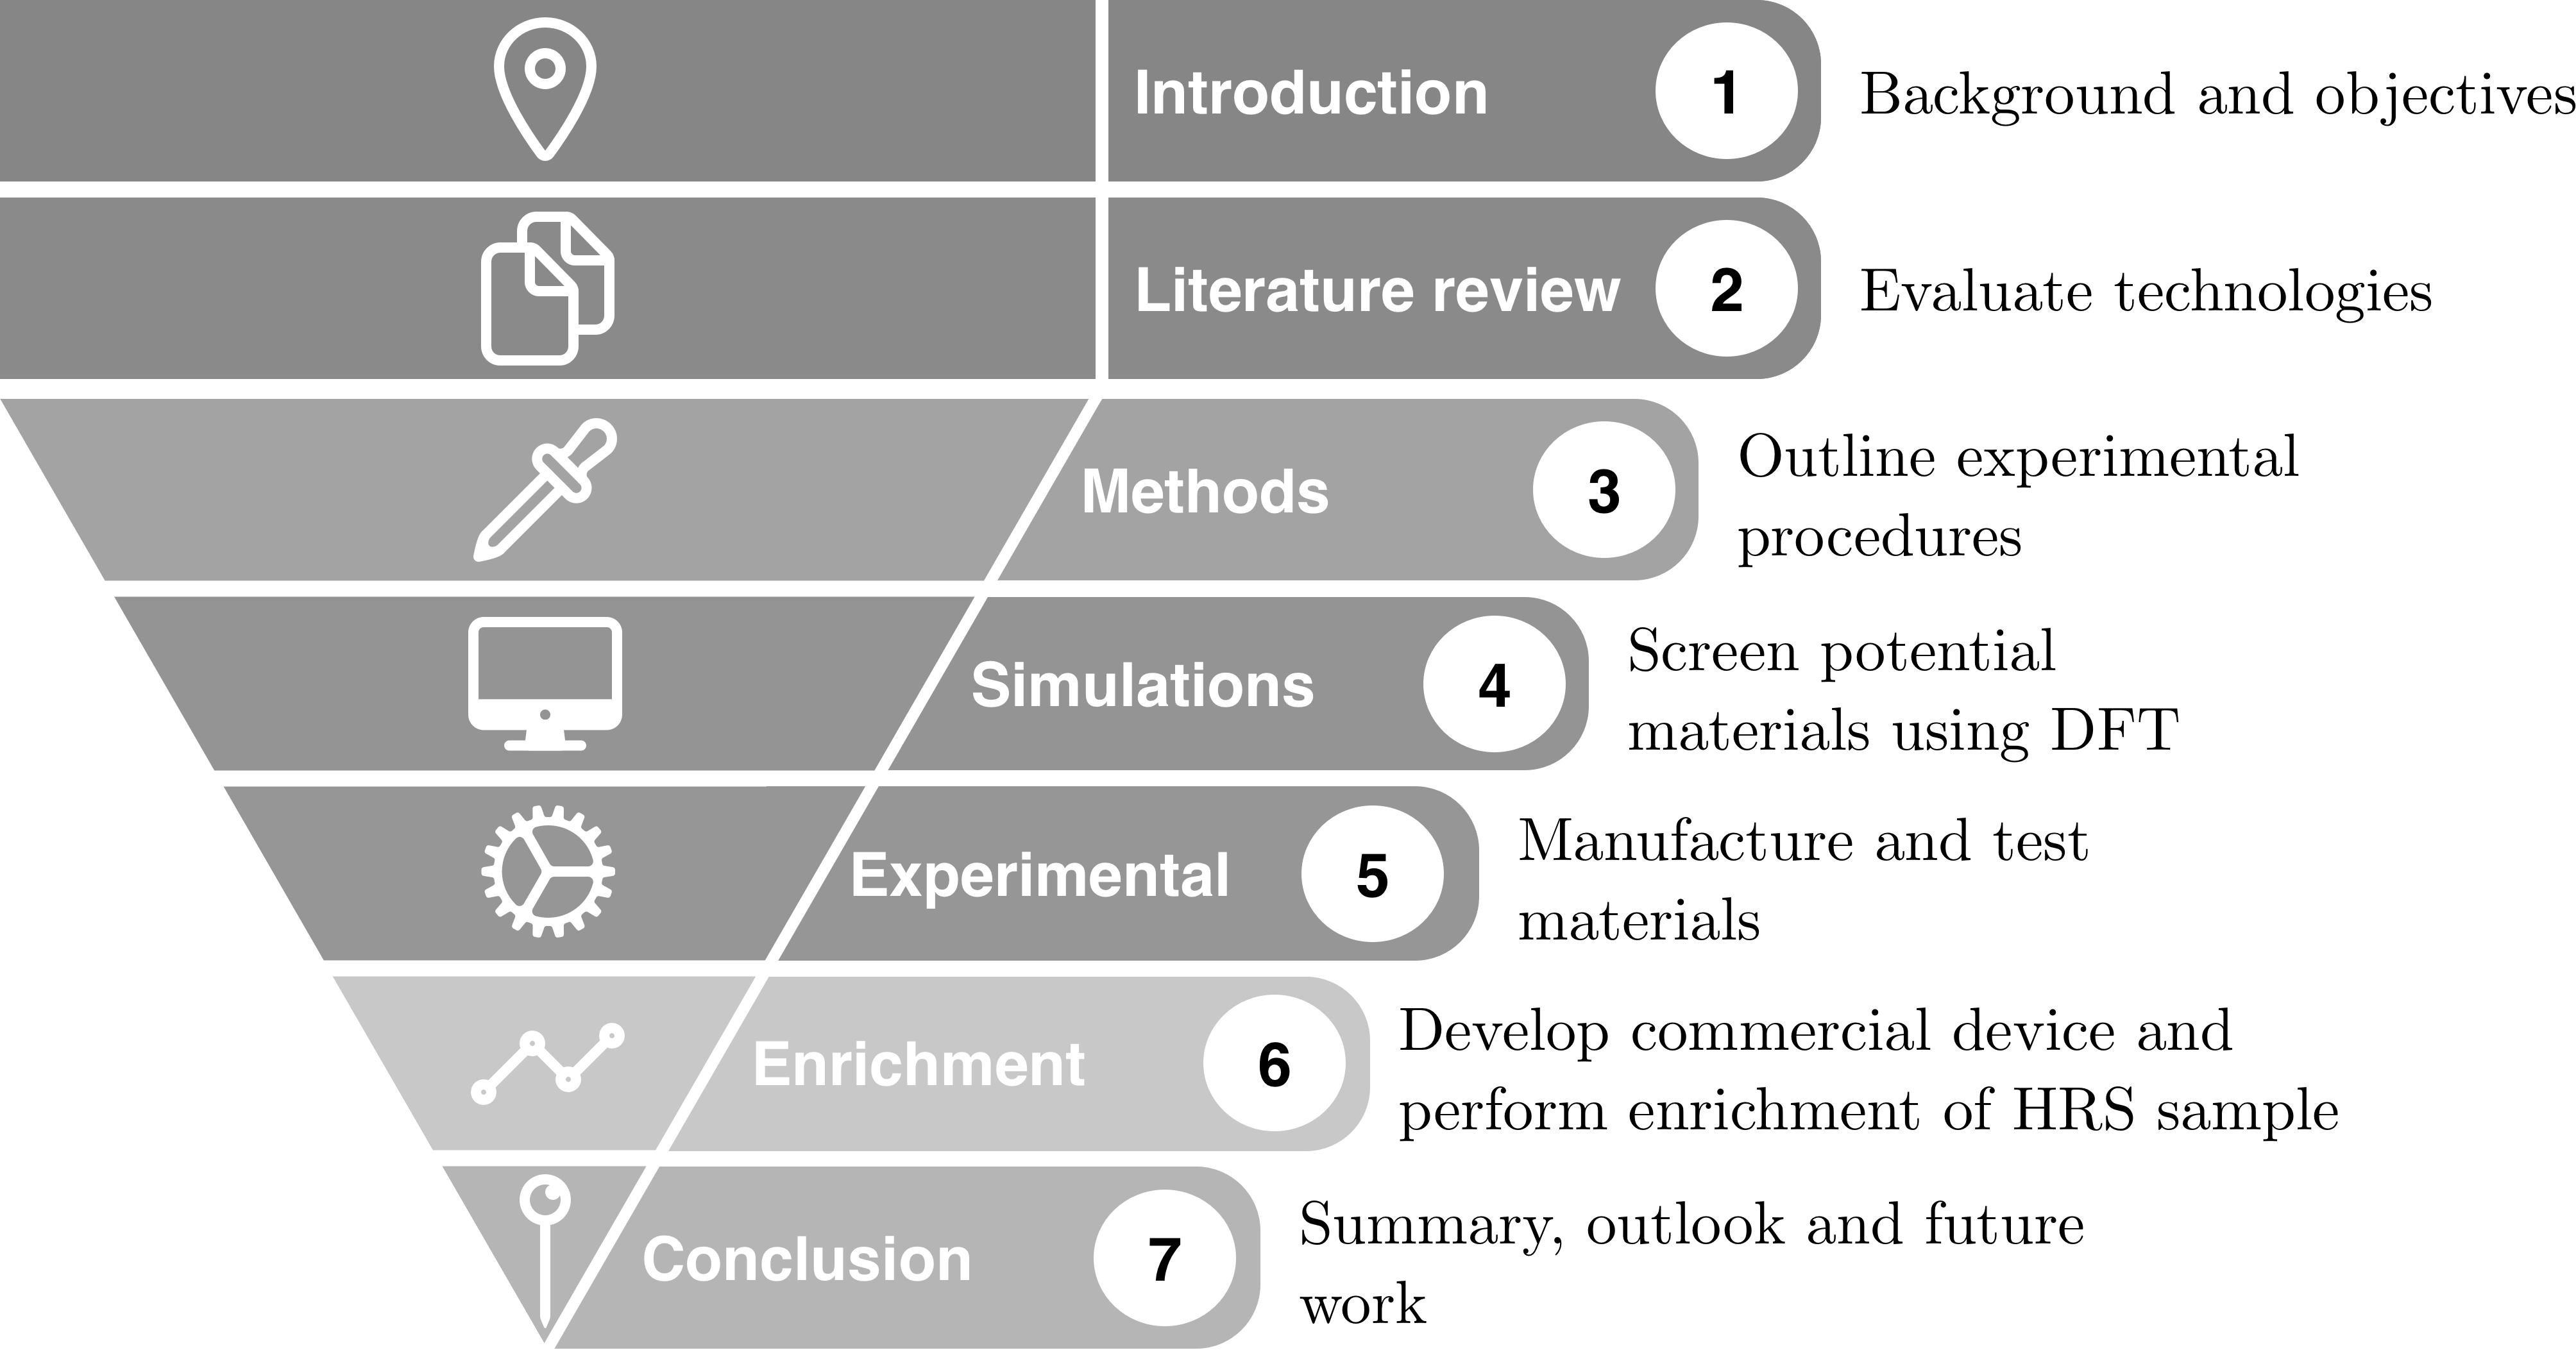
\includegraphics[width=\linewidth]{figures/funnel.png}
  \caption{Schematic presentation of the thesis structure}
  \label{funnel}
\end{figure}


\renewcommand{\bibname}{References}
\bibliographystyle{unsrtnat}
\bibliography{library.bib}